\documentclass[12pt]{article}
\usepackage{amsmath, amssymb, amsthm}
\usepackage{mathtools}
\usepackage{graphicx}
\usepackage{float}
\usepackage{hyperref}
\usepackage{xcolor}
\usepackage{listings}
\usepackage{geometry}
\usepackage{algorithm}
\usepackage{algpseudocode}
\usepackage{tikz}
\usepackage{longtable}
\usepackage{circuitikz}
\usepackage{comment}
\usepackage{MnSymbol}
\usepackage{physics}
\usepackage[section]{placeins}

\providecommand{\brak}[1]{\ensuremath{\left(#1\right)}}
\geometry{a4paper, margin=1in}

\title{Damped LC 
\author{Abhimanyu Koushik \brak{\text{EE24BTECH11024}},\\Agamjot Singh \brak{\text{EE24BTECH11002}}\\IIT Hyderabad}Oscillations}
\date{\today}

\begin{document}

\maketitle

\begin{abstract}
    This report explores the behavior of an RLC circuit exhibiting damped oscillations. The differential equation governing the circuit is derived, and solutions for different damping conditions are analyzed. Simulations and plots illustrate the circuit's response.
\end{abstract}

\section{Introduction}
An LC circuit consists of an inductor (L) and a capacitor (C), forming an oscillatory system. When a resistor (R) is added, the circuit exhibits damped oscillations, leading to energy dissipation over time.

\section{Theory for Underdamped Case}
\begin{figure*}[h]
    \begin{center}
        \begin{circuitikz}
            \draw
            (0,0) to[C, l=$C$] (0,3)
            to (3,3)
            to[R, l=$R$] (3,1.5)
            to[L, l=$L$] (3,0)
            to (0,0);
        \end{circuitikz}
    \end{center}
\end{figure*}
Taking Kirchhoff's law in the circuit loop gives the equation 
\begin{align*}
    L\frac{di}{dt} + iR + \frac{1}{C}\int_{}^{}idt &= 0\\
    L\frac{d^2q}{dt^2} + R\frac{dq}{dt} + \frac{q}{C} &= 0\\
    \frac{d^2q}{dt^2} + \frac{R}{L}\brak{\frac{dq}{dt}} + \frac{q}{LC} &= 0
\end{align*}
\newpage
This equation can be written as,
\begin{align*}
    \frac{d^2q}{dt^2} + 2\xi\omega_{n}\brak{\frac{dq}{dt}} + \omega_{n}\frac{q}{LC} &= 0
\end{align*}
where $\xi$ is the damping factor, $\xi = \frac{R}{2}\sqrt{\frac{C}{L}}$, and $\omega_{n}$ is the natural frequency, $\omega_{n} = \frac{1}{\sqrt{LC}}$.
\newline

According to the initial conditions, the initial current in the circuit is 0 and the initial voltage across capacitor is $V_{C_0}$ which gives $\frac{dq}{dt}\Bigr|_{t=0} = 0 $ and $q(0) = CV_{C_0}$.

The solution to the given differential equation can be given by,
\begin{align*}
    q = c_1e^{s_1 t} + {c_2} e^{s_2 t}
\end{align*}

where $s_1, s_2$ are the solutions for the quadratic equation $s^2 + 2\xi\omega_{n}s + \brak{\omega_{n}}^2 = 0$ and $c_1, c_2$ are constants.

For an underdamped system ($\xi < 1$),
\begin{align*}
    s_2 &= {s_1}^{\ast} = s^{\ast}\\
    c_2 &= {c_1}^{\ast} = c^{\ast}\\
    \implies q &= ce^{st} + c^{\ast}e^{s^{\ast}t}
\end{align*}
Let $c = a+ib$ then
\begin{align*}
  s = -\xi\omega_n \pm \omega_n\sqrt{\xi^2-1}\\
  s = -\xi\omega_n \pm i\omega_n\sqrt{1-\xi^2}\\
  q\brak{0} = ce^{0s} + c^{\ast}e^{0s^{\ast}}\\
  q\brak{0} = c + c^{\ast}\\
  q\brak{0} = 2a\\
  a = \frac{CV_{C_0}}{2}\\
  q^{\prime}\brak{0} = cs + c^{\ast}s^{\ast}\\
  \brak{a+ib}\brak{-\xi\omega_n + i\omega_n\sqrt{1-\xi^2}} + \brak{a-ib}\brak{-\xi\omega_n - i\omega_n\sqrt{1-\xi^2}} = 0\\
  -a\xi\omega_n - b\omega_n\sqrt{1-\xi^2} = 0\\
  b = \frac{-a\xi}{\sqrt{1-\xi^2}}\\
  b = \frac{-CV_{C_0}\xi}{2\sqrt{1-\xi^2}}
\end{align*}
Substituting the value of $a$ and $b$ gives
\begin{align*}
  q\brak{t} = e^{-\xi\omega_n t}\brak{\brak{a+ib}e^{i\omega_n t\sqrt{1-\xi^2}} + \brak{a-ib}e^{-i\omega_n t\sqrt{1-\xi^2}}}\\
  q\brak{t} = e^{-\xi\omega_n t}\brak{2a\cos\brak{\brak{\omega_n\sqrt{1-\xi^2}}t} - 2b\sin\brak{\brak{\omega_n\sqrt{1-\xi^2}}t}}\\
  q\brak{t} = e^{-\xi\omega_n t}\brak{CV_{C_0}\cos\brak{\brak{\omega_n\sqrt{1-\xi^2}}t} + \frac{CV_{C_0}\xi}{\sqrt{1-\xi^2}}\sin\brak{\brak{\omega_n\sqrt{1-\xi^2}}t}}\\
 \end{align*}

\section{Solution for Underdamped Case}
For $\xi < 1$, the general solution is:\newline
$V\brak{t} = V_{C_0}e^{-\xi\omega_n t}\brak{\cos\brak{\brak{\omega_n\sqrt{1-\xi^2}}t} + \frac{\xi}{\sqrt{1-\xi^2}}\sin\brak{\brak{\omega_n\sqrt{1-\xi^2}}t}}$
\section{Procedure}
\begin{enumerate}
    \item Connect the circuit as per the circuit diagram.
    \item Measure the internal resitance of the inductor using a multimeter.
    \item Oscilloscope's probes are to be connected across the inductor to measure the voltage across it. Set the display mode to $X - T$.
    \item Disconnect the capacitor and inductor to charge the capacitor.
    \item Use a Regulated DC Supply to provide $5 V$ DC voltage across the capacitor.
    \item Disconnect the voltage supply and connect the inductor back to the capacitor, one after the other. 
    \item Measure the Voltage drop across the capacitor using the Oscilloscope probe. Capture the wave which is being displayed on the screen. It is the graph of the response in steady state.
    \item Enter the \textbf{Cursor} menu and set the cursor $A$ to the current channel. Use the knob marked as $\lcirclearrowright$ to adjust the marker.
    \item To check the voltage value, check the marker value at the maximum point of output wave.
\end{enumerate}

\section{Simulation and Results}
Numerical simulations were conducted using Python to visualize the circuit response.
\begin{align}
    R &= 24.5\,\Omega \text{ (internal resistance of inductor)}\\
    L &= 2.2\,mH\\ 
    C &= 460\,pF
\end{align}
Oscilloscope $\hspace{\fill}$ Simulation $\hspace{1in}$
\FloatBarrier
\begin{figure*}[!htb]
    {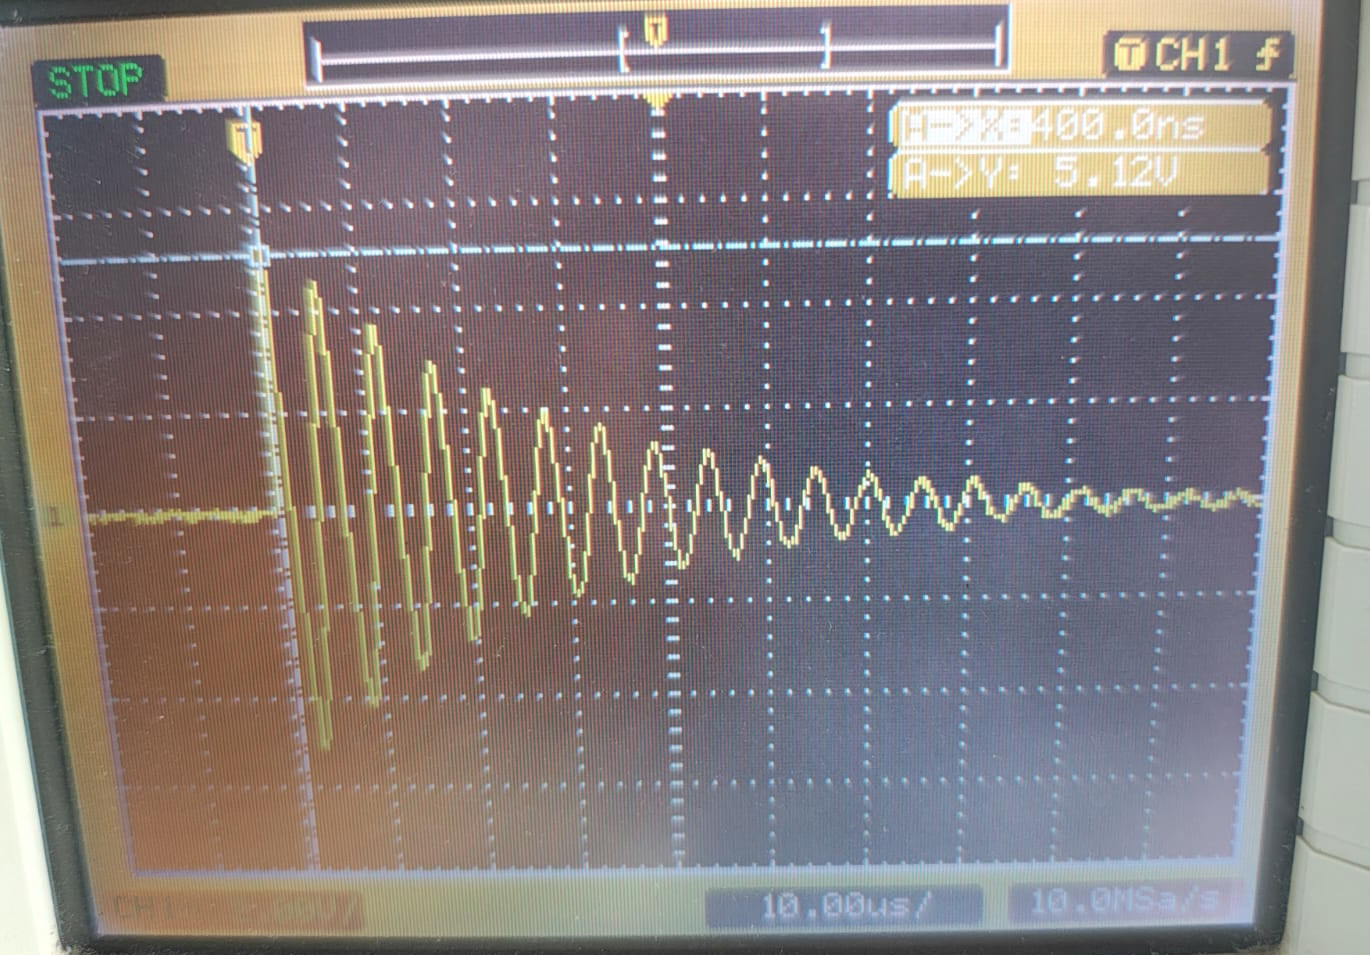
\includegraphics[ width=0.5\textwidth]{./figs/rlc_real.jpeg}}
    \hspace{\fill}
    {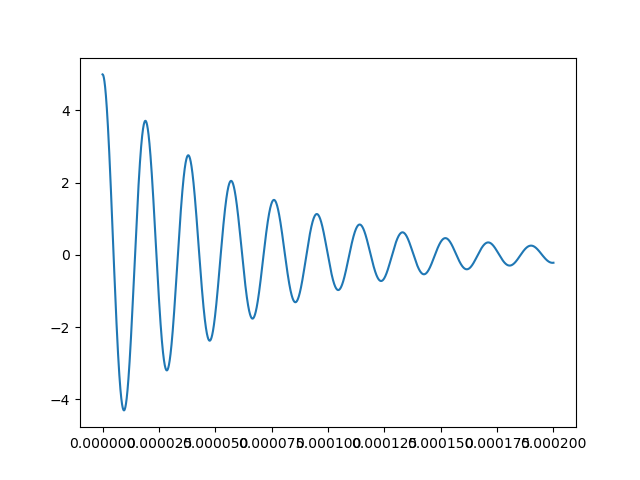
\includegraphics[ width=0.5\textwidth]{./figs/rlc.png}}
\end{figure*}

\section{Verification Codes}
Python verification codes are provided below,
\newline
\url{https://github.com/AbhimanyuKoushik/EE1200/blob/main/Lab4/codes/rlc.py}

\section{Conclusion}
Damped LC circuits exhibit different responses based on resistance. Understanding these behaviors is crucial in designing stable electronic systems.

\end{document}
